\section{Relationship Modeling Networks}
\label{sec:model}

\begin{figure}[t!]
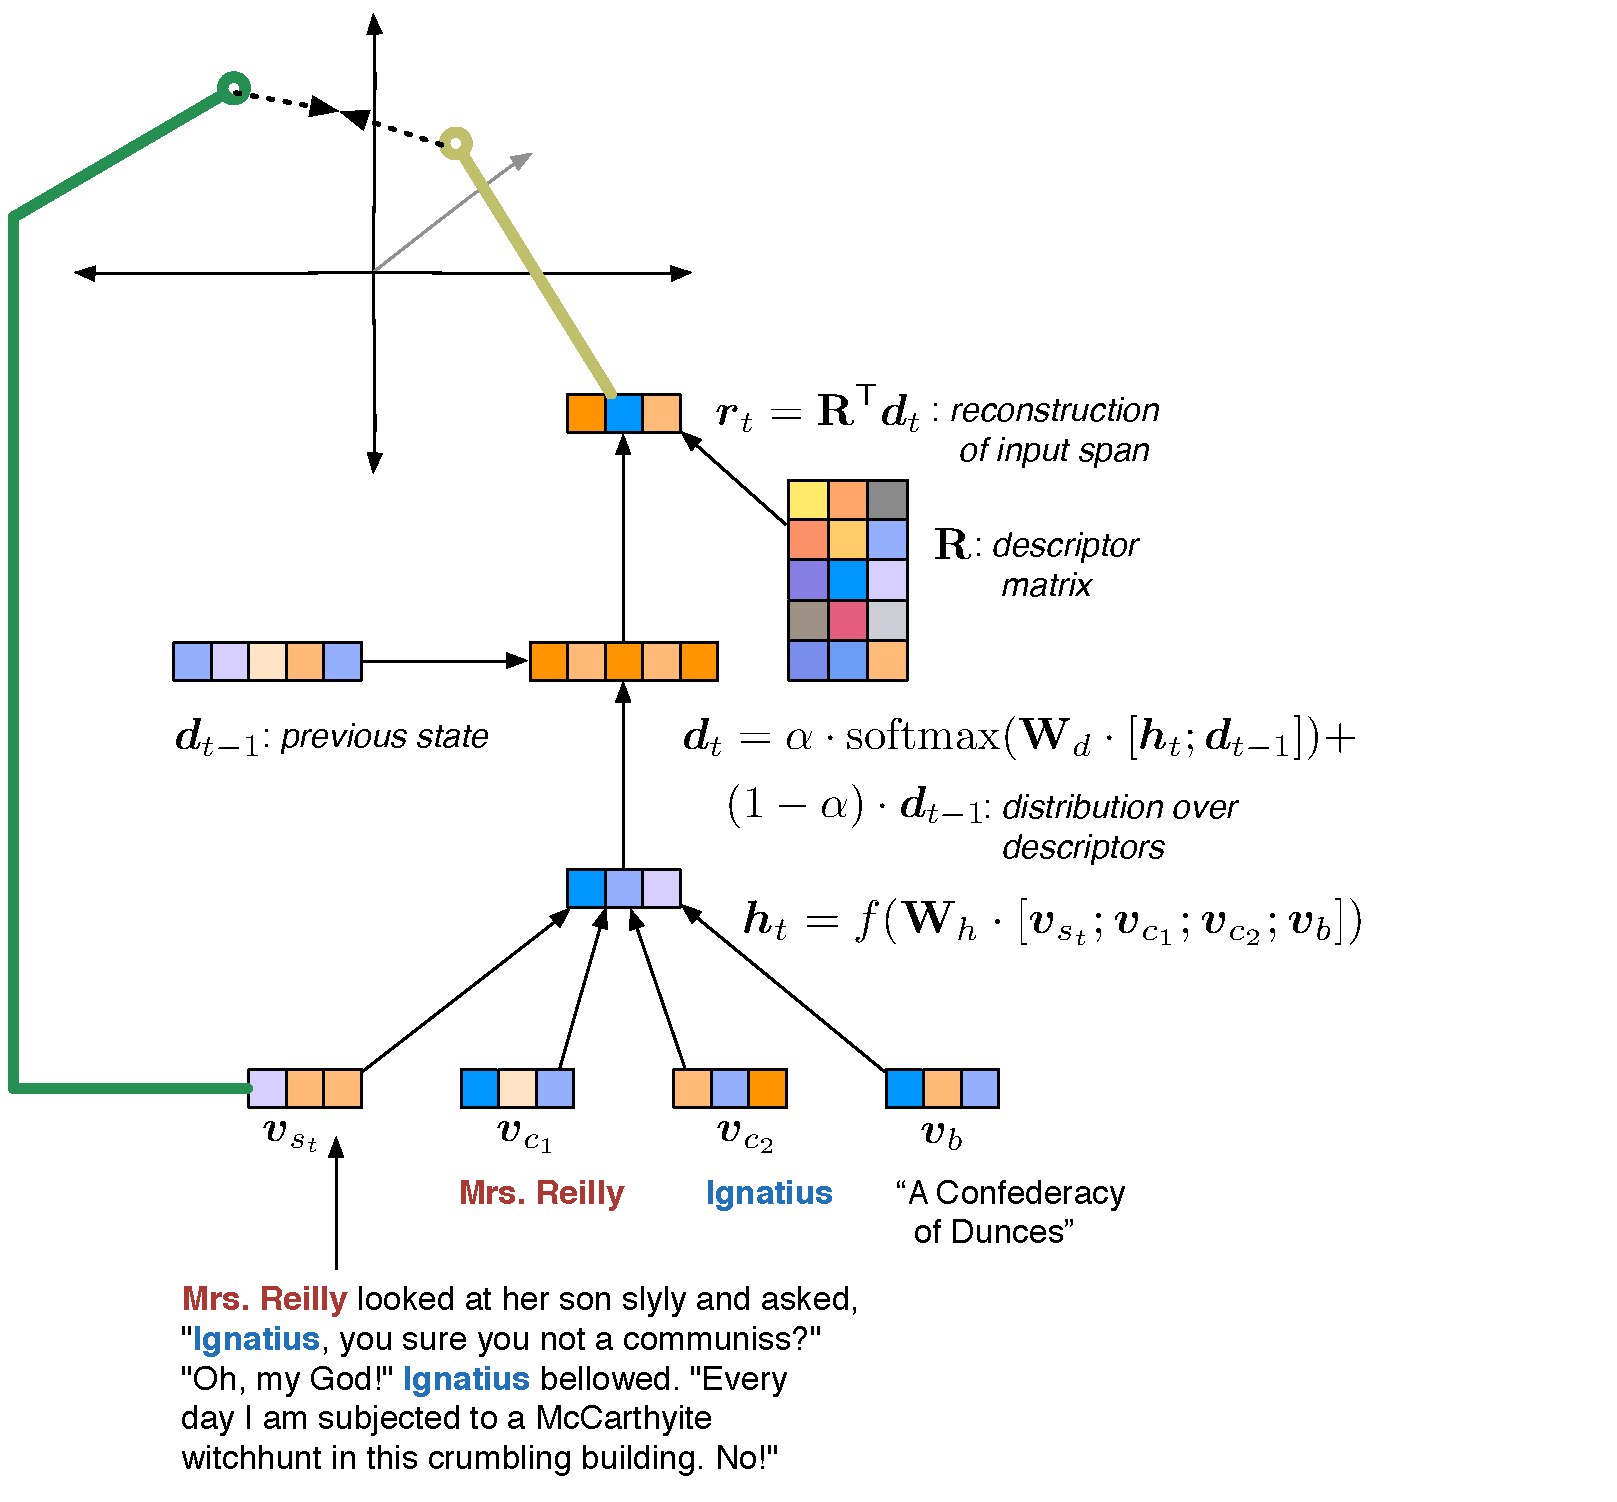
\includegraphics[width=1.15\linewidth]{2016_naacl_relationships/figures/rmn.pdf}
\caption{An example of the \rmn's computations at a single time step. The model
  approximates the vector average of an input span ($\bvec{v}_{s_t}$) as a
  linear combination of descriptors from \bmat{R}. The descriptor weights
  $\bvec{d}_t$ define the relationship state at each time step and---when viewed
  as a sequence---form a relationship trajectory.}
\label{fig:rmn}
\end{figure}

This section mathematically describes how we apply the \rmn\ to relationship
modeling on our dataset. Our model is similar in spirit to topic models: for an
input dataset, the output of the \rmn\ is a set of relationship descriptors
(topics) and---for each relationship in the dataset---a trajectory, or a
sequence of probability distributions over these descriptors (document-topic
assignments). However, the \rmn\ uses recent advances in deep learning to
achieve better control over descriptor coherence and trajectory smoothness
(Section~\ref{sec:experiments}).

\subsection{Formalizing the Problem}

Assume we have two characters $c_1$ and $c_2$ in book~$b$. We define
$S_{c_1, c_2}$ as a sequence of token spans where each span $s_t \in
S_{c_1, c_2}$ is itself a set of tokens $\{w_1, w_2, \dots, w_l\}$ of
fixed size~$l$ that contains mentions (either directly or by
coreference) to both $c_1$ and $c_2$. In other words, $S_{c_1, c_2}$
includes the text of every scene, chronologically ordered, in which
$c_1$ and $c_2$ are present together.

\subsection{Model Description}

As in other neural network models for natural language processing, we
begin by associating each word type \emph{w} in our vocabulary with a
real-valued embedding $\bvec{v}_w \in \mathbbm{R}^d$. These embeddings
are rows of a $V \times d$ matrix \bmat{L}, where $V$ is the
vocabulary size. Similarly, characters and books have their own
embeddings in rows of matrices \bmat{C} and \bmat{B}. We want
\bmat{B} to capture global context information (e.g., ``Moby Dick''
takes place at sea) and \bmat{C} to capture immutable aspects of
characters not related to their relationships (e.g., Javert is a
police officer). Finally, the \rmn\ learns embeddings for
relationship descriptors, which requires a second matrix \bmat{R} of
size $K \times d$ where $K$ is the number
of descriptors, analogous to the number of topics in topic models.

Each input to the \rmn\ is a tuple that contains identifiers for a book and two
characters, as well as the spans corresponding to their relationship: $(b, c_1,
c_2, S_{c_1,c_2})$. Given one such input, our objective is to reconstruct
$S_{c_1,c_2}$ using a linear combination of relationship descriptors from
\bmat{R} as shown in Figure~\ref{fig:rmn}; we now describe this process
formally.

\subsubsection{Modeling Spans with Vector Averages}

We compute a vector representation for each span $s_t$ in $S_{c_1,c_2}$ by
averaging the embeddings of the words in that span,
\begin{equation}\label{eq:ave}
\bvec{v}_{s_t} = \frac 1 {l} {\sum_{w \in s_t} \bvec{v}_w}.
\end{equation}
Then, we concatenate $\bvec{v}_{s_t}$ with the character
embeddings~$\bvec{v}_{c_1}$ and $\bvec{v}_{c_2}$ as well as the book embedding
$\bvec{v}_b$ and feed the resulting vector into a standard feed-forward layer to
obtain a hidden state~$\bvec{h}_t$,
\begin{equation}\label{eq:dan}
	\bvec{h}_t = f(\bmat{W}_h\cdot [\bvec{v}_{s_t};\bvec{v}_{c_1};\bvec{v}_{c_2};\bvec{v}_{b}]).
\end{equation}
In all experiments, the transformation matrix $W_h$ is
$d \times 4d$, and we set $f$ to the $\mbox{ReLu}$ function,
$\mbox{ReLu}(x) = \mathrm{max}(0, x)$.

\subsubsection{Approximating Spans with Relationship Descriptors}

Now that we can obtain representations of spans, we move on to
learning descriptors using a variant of dictionary
learning~\cite{olshausen1997sparse,elad2006image}, where our descriptor matrix \bmat{R}
is the dictionary and we are trying to approximate input spans as a
linear combination of items from this dictionary.













Suppose we compute a hidden state for every span $s_t$ in $S_{c_1,c_2}$
(Equation~\ref{eq:dan}). Now, given an $\bvec{h}_t$, we compute a weight vector
$\bvec{d}_t$ over $K$ relationship descriptors with some composition function
$g$, which is fully specified in the next section. Conceptually, each
$\bvec{d}_t$ is a \emph{relationship state}, and a \emph{relationship
  trajectory} is a sequence of chronologically-ordered relationship states as
shown in Figure~\ref{fig:traj}. After computing $\bvec{d}_t$, we use it to
compute a reconstruction vector~$\bvec{r}_t$ by taking a weighted average over
relationship descriptors,
\begin{equation}\label{eq:recon}
	\bvec{r}_t = \bmat{R}^\mathsf{T} \bvec{d}_t.
\end{equation}
Our goal is to make $\bvec{r}_t$ similar to $\bvec{v}_{s_t}$. We use a
contrastive max-margin objective function similar to previous
work~\cite{weston2011wsabie,sochergrounded}. We randomly sample spans from our
dataset and compute the vector average $\bvec{v}_{s_n}$ for each sampled span as
in Equation~\ref{eq:ave}. This subset of span vectors is $N$. The unregularized
objective~$J$ is a hinge loss that minimizes the inner product between
$\bvec{r}_t$ and the negative samples while simultaneously maximizing the inner
product between $\bvec{r}_t$ and $\bvec{v}_{s_t}$,
\begin{equation}\label{eqn:obj}
J(\theta) = \sum\limits_{t=0}^{\norm{S_{c_1,c_2}}}\sum\limits_{n \in
  N} \mathrm{max}(0, 1 - \bvec{r}_t\bvec{v}_{s_t} +
\bvec{r}_t\bvec{v}_{s_n}),
\end{equation}
where $\theta$ represents the model parameters.

\subsubsection{Computing Weights over Descriptors}

What function should we choose for our composition function~$g$ to represent a
relationship state at a given time step?  On the face of it, this seems trivial;
we can project $h_t$ to $K$ dimensions and then apply a softmax or some other
nonlinearity that yields non-negative weights.\footnote{We experiment with a
  variety of nonlinearities but find that the softmax yields the most
  interpretable results due to its predisposition to select a single
  descriptor.} However, this method ignores the relationship states at previous
time steps. To model the temporal aspect of relationships, we can add a
recurrent connection,
\begin{equation}\label{eq:rnn}
	\bvec{d}_t = \mbox{softmax}(\bmat{W}_d\cdot [\bvec{h}_t;\bvec{d}_{t-1}])
\end{equation}
where $\bmat{W}_d$ is of size $K\times (d+K)$ and
$\mbox{softmax}(\bvec{q}) = \nicefrac{\exp{\bvec{q}}}{\sum_{j=1}^k
  \exp{\bvec{q}_j}}$.

Our hope is that this recurrent connection will carry some of the previous
relationship state over to the current time step. It should be unlikely for two
characters in love at time $t$ to fall out of love at time $t+1$ even if
$s_{t+1}$ does not include any love-related words.  However, because the
objective function in Equation~\ref{eqn:obj} maximizes similarity with the
current time step's input, the model is not forced to learn a smooth
interpolation between the previous state and the current one. A natural remedy
is to have the model predict the \emph{next} time step's input instead, but this
proves hard to optimize.













We instead \emph{force} the model to use the previous relationship state by
modifying Equation~\ref{eq:rnn} to include a linear interpolation
between $\bvec{d}_{t}$ and $\bvec{d}_{t-1}$,
\begin{equation}\label{eq:rmn}
\begin{split}
	\bvec{d}_t &= \alpha \cdot \text{softmax}(\bmat{W}_d\cdot [\bvec{h}_t;\bvec{d}_{t-1}]) + \\&(1-\alpha)\cdot \bvec{d}_{t-1}.
\end{split}
\end{equation}
Here, $\alpha$ is a scalar between $0$ and $1$. We experiment with
setting $\alpha$ to a fixed value of $0.5$ as well as allowing the
model to learn $\alpha$ as in
\begin{equation}\label{eq:alpha}
	\alpha = \sigma(\bvec{v}_\alpha^\mathsf{T} \cdot[\bvec{h}_t;\bvec{d}_{t-1};\bvec{v}_{s_t}]),
\end{equation}
where $\sigma$ is the sigmoid function and $\bvec{v}_\alpha$ is a vector of
dimensionality $2d+K$.  Fixing $\alpha=0.5$ initially and then tuning it after
other parameters have converged improves training stability; for the specific
hyperparameters we use see Section~\ref{sec:experiments}.\footnote{This strategy
  is reminiscent of alternative minimization strategies for dictionary
  learning~\cite{agarwallearning}, where the dictionary and weights are learned
  separately by keeping the other fixed.}

\subsubsection{Interpreting Descriptors and Enforcing Uniqueness}
Recall that each descriptor is a $d$-dimensional row of
\bmat{R}. Because our objective function $J$ forces these descriptors
to be in the same vector space as that of the word embeddings \bmat{L}, we can
interpret them by looking at nearest neighbors in \bmat{L} using
cosine distance as the similarity metric.

To discourage learning descriptors that are too similar to
each other, we add another penalty term $X$ to our objective function,
\begin{equation}\label{eq:unique}
	X(\theta) = \euclidean{\bmat{R}\bmat{R}^\mathsf{T} - \bmat{I}},
\end{equation}
where \bmat{I} is the identity matrix. This term comes from
the component orthogonality constraint in independent component
analysis~\cite{hyvarinen2000independent}.

We add $J$ and $X$ together to obtain our final training objective $L$,
\begin{equation}\label{eq:final}
	L(\theta) = J(\theta) + \lambda X(\theta),
\end{equation}
where $\lambda$ is a hyperparameter that controls the magnitude of the
uniqueness penalty.
